%\documentclass[letter,11pt]{article} % Tamaño de página y letra, tipo de documento
%\usepackage[top = 2.0cm, bottom = 2.0cm, left = 2.0cm, right = 2.0cm]{geometry}

\documentclass[letter,11pt]{article}
\usepackage[top=2.0cm, bottom=2.0cm, left=2.0cm, right=2.0cm]{geometry}

% Configuración de Fira Sans para TODO el documento
\usepackage[sfdefault]{FiraSans} % Fuente principal
\usepackage{FiraMono}

%% Comandos para codificación de archivo
%\usepackage[T1]{fontenc}
\usepackage[utf8]{inputenc}
% Se configura diccionario en español y en entorno de tablas aparecerá el nombre Tabla x
\usepackage[spanish,es-tabla]{babel}
% Se utilizará el punto decimal en lugar de coma para definir números con decimales
\spanishdecimal{.}
%%%%%%%%%%%%%%%%%%%%%%%%%%%%%%%%%%%%%%%%%%%%%%%%
%% Bibliotecas útiles %%
\usepackage{multirow} % Múltiples renglones
\usepackage{multicol} % Múltiples columnas
\usepackage{booktabs} % For even nicer tables.
\usepackage{graphicx} % Necesario para agregar figuras
\usepackage{setspace}  % Quita sangría de inicio de párrafos
\setlength{\parindent}{0in}
\usepackage{float} % Colocar figuras donde se indique
\usepackage{fancyhdr} % Da formato a encabezados
\usepackage{amsmath,mathtools,amsfonts,amssymb} % Para agregar símbolos matemáticos
\usepackage{epstopdf} % Para agregar figuras en formato eps
\usepackage{xcolor} % Para agregar color a texto y ecuaciones
\usepackage{fancyvrb}  % Necesario para incluir código de Matlab
\usepackage{pdfpages}
\usepackage[T1]{fontenc}     % Para mejor soporte de fuentes
\usepackage{enumitem}
\usepackage{subcaption}
\usepackage{tocloft}
\usepackage{hyperref}
\usepackage{array}
\usepackage{tcolorbox}
\usepackage{siunitx}
\usepackage{lmodern}
\usepackage{tikz}
\usepackage{circuitikz}
\usepackage{geometry}
\usepackage{anyfontsize}
\usepackage{fancybox}
\usepackage[normalem]{ulem}
\hypersetup{
	colorlinks=false,
	pdfborder={0 0 0}
}
\usepackage{listings}
\definecolor{backcolour}{rgb}{0.95,0.95,0.92}

\lstdefinestyle{bashstyle}{
	backgroundcolor=\color{backcolour},
	basicstyle=\ttfamily\small,
	numbers=left,
	numberstyle=\tiny\color{gray},
	frame=single,
	tabsize=4,
	breaklines=true,
	captionpos=b,
	keywordstyle=\color{blue},
	commentstyle=\color{green!50!black},
	stringstyle=\color{red},
	morekeywords={sudo, apt, git, echo, if, then, else, fi, for, do, done, while, until, case, esac, function, cd, ls, mkdir, rm, cp, mv, chmod, grep, find, awk, sed},
	literate=*
	{_} {\textunderscore}{1}  % ← Esto arregla el guión bajo
	{\$} {\textdollar}{1}
	{\#} {\#}{1}
	{\{} {\{}{1}
	{\}} {\}}{1}
	{>} {\textgreater}{1}
	{<} {\textless}{1}
	{|} {\textbar}{1}
	{~} {\textasciitilde}{1}
	{\`} {\`}{1}
	{\^} {\^{}}{1}
	{*} {\ast}{1}
}

\lstdefinestyle{sqlstyle}{
	language=SQL,
	basicstyle=\ttfamily\small,
	keywordstyle=\color{blue},
	commentstyle=\color{green!60!black}, % Verde más oscuro/menos fosforescente
	stringstyle=\color{red},
	numbers=left,
	numberstyle=\tiny,
	stepnumber=1,
	numbersep=5pt,
	breaklines=true,
	frame=single,
	literate= % Para aceptar tildes y caracteres especiales
	{á}{{\'a}}1 {é}{{\'e}}1 {í}{{\'i}}1 {ó}{{\'o}}1 {ú}{{\'u}}1
	{Á}{{\'A}}1 {É}{{\'E}}1 {Í}{{\'I}}1 {Ó}{{\'O}}1 {Ú}{{\'U}}1
	{ñ}{{\~n}}1 {Ñ}{{\~N}}1
}

% Definir estilo sutil con bordes redondeados
\newtcbox{\highlight}[1][]{%
	nobeforeafter,
	tcbox raise base,
	arc=3pt,
	boxrule=0pt,
	left=2pt,
	right=2pt,
	top=1pt,
	bottom=1pt,
	colback=yellow!20!white,
	colframe=white,
	#1
}

% Colores institucionales UNAM
\definecolor{unamblue}{RGB}{0,51,102}
\definecolor{unamgold}{RGB}{153,126,48}
\definecolor{myred}{HTML}{911010}
\definecolor{myblue}{HTML}{142966}
\definecolor{myaqua}{HTML}{1EA69A}


%% Encabezado y pie de página %%
\pagestyle{fancy}  
\fancyhf{} 
\renewcommand{\headrule}{\hbox to\headwidth{\color{black}\leaders\hrule height \headrulewidth\hfill}}
\renewcommand{\headrulewidth}{0.4pt} % Línea del encabezado
\fancyhead[L]{\color{black}\small{Laboratorio de Circuitos Eléctricos}}
\fancyhead[R]{\color{black}\small{Reporte de Práctica 1}}
\fancyfoot[R]{\small\thepage}
\fancyfoot[L]{Brigada 1B - Díaz Antúnez, Trejo Olvera}

%%%%%%%%%%%%%%%%%%%%%%%%%%%%%%%%%%%%%%%%%%%%%%%%
%% Aquí comienza la edición del documento

\begin{document}
	\thispagestyle{empty} % Sin encabezado la primera página
	%% Datos para la primera página
	\begin{center}
		\vspace{0.8cm}
		\begin{minipage}{0.125\textwidth}
			\centering
			
\includegraphics[width=\textwidth]{UNAM}
		\end{minipage}
		\hfill
		\begin{minipage}{0.7\textwidth}
			\centering
			{\color{black}\fontsize{16}{18}\selectfont
				\textbf{UNIVERSIDAD NACIONAL AUTÓNOMA DE MÉXICO} \\
				\vspace{0.3cm}
				\textbf{FACULTAD DE INGENIERÍA} \\
				\vspace{0.3cm}
				\textbf{LABORATORIO DE CIRCUITOS ELÉCTRICOS} \\
				\vspace{0.3cm}
				\textbf{SEMESTRE 2026 - 2}
			}
		\end{minipage}
		\hfill
		\begin{minipage}{0.125\textwidth}
			\centering
			
\includegraphics[width=\textwidth]{UNAM_INGENIERIA}
		\end{minipage}
		
		\vspace{2cm}
		
		\begin{tikzpicture}
			%\draw[unamgold, line width=1pt] (0,0) -- (0.2\textwidth,0);
			%\draw[unamblue, line width=1pt] (0.2\textwidth,0) -- (0.8\textwidth,0);
			\draw[black, line width=1.5pt] (2\textwidth,0) -- (\textwidth,0);
		\end{tikzpicture}
		
		\vspace{2cm}
		
		{\color{black}\fontsize{18}{20}\selectfont
			\textbf{REPORTE DE PRÁCTICA 1} \\
			\vspace{0.5cm}
			\textbf{EXCITACIÓN EN AC Y DC, PARA CIRCUITOS RC Y RL}
		}
		
		\vspace{1.5cm}
		
		{\color{black}\fontsize{14}{16}\selectfont
			\begin{tabular}{l r}
				\textbf{NO. BRIGADA} & \textit{1B} \\[0.3cm]
				\textbf{INTEGRANTES} & \textit{Díaz Antúnez David, Trejo Olvera Emmanuel} \\[0.3cm]
				\textbf{PROFESOR} & \textit{Ing. Julio Serrano Villegas} \\[0.3cm]
				\textbf{GRUPO} & \textit{04} \\[0.3cm]
				\textbf{FECHA DE ENTREGA} & \textit{11 de marzo de 2026}
			\end{tabular}
		}
		
		\vfill
		
		{\color{black}\fontsize{12}{14}\selectfont
			Ciudad Universitaria, CDMX \hfill 11 de marzo de 2026
		}
	\end{center}
	
	\newpage
	\vspace*{0.5cm} 
	\hfill {\Large \bf {\LARGE EXCITACIÓN EN AC Y DC, PARA CIRCUITOS RC Y RL}} 
	\renewcommand{\contentsname}{Contenido}
	\setlength{\cftbeforetoctitleskip}{0pt}
	\tableofcontents
	\thispagestyle{fancy}
	\newpage
	
\section{Introducción}
	
	El estudio de los circuitos eléctricos en ingeniería requiere comprender tanto el comportamiento transitorio como el de régimen permanente. 
	El objetivo principal de este análisis es entender la respuesta en frecuencia de sistemas lineales e invariantes en el tiempo (LTI),
	así como calcular las variables eléctricas y los desfases que ocurren en circuitos de primer orden, 
	específicamente los de tipo RC y RL.
	
	\hspace{0.5cm}Un sistema de primer orden se caracteriza por tener una dinámica descrita por una ecuación diferencial lineal de primer orden, lo cual es fundamental para modelar circuitos que contienen un solo elemento de almacenamiento de energía y elementos resistivos (resistencias).
	En estos sistemas, la constante de tiempo $\tau$ dicta la rapidez con la que el circuito reacciona ante cambios de voltaje o corriente, siendo el tiempo necesario para alcanzar el $63.2\%$ de su valor final.
	
	\hspace{0.5cm}Por otro lado, cuando los circuitos son excitados por fuentes senoidales, el análisis se traslada al dominio de la impedancia compleja y la notación fasorial. La impedancia permite establecer la relación entre la tensión y la intensidad de corriente, considerando no solo su magnitud sino también el ángulo de fase provocado por elementos pasivos como inductores y capacitores.
	
	\hspace{0.5cm}En esta práctica se estudiará el comportamiento dinámico y estacionario de los circuitos RC y RL al ser expuestos a diferentes condiciones de excitación, como pueden ser las señales senoidales y señales cuadradas.
	El análisis se centrará en observar cómo estos sistemas responden ante cambios bruscos de tensión (análisis transitorio) y cómo se comportan una vez que alcanzan la estabilidad (régimen permanente), permitiendo validar de forma experimental los conceptos de almacenamiento de energía en campos eléctricos y magnéticos.
	
	\hspace{0.5cm}Así mismo, se buscará determinar la relación que existe entre los componentes pasivos y la rapidez de respuesta del sistema. 
	A través del uso de herramientas de medición como el osciloscopio, se identificarán los desfasamientos entre la tensión y la corriente, así como las variaciones en la impedancia del circuito al modificar la frecuencia de la fuente de alimentación, consolidando así los fundamentos del análisis en el dominio del tiempo y de la frecuencia.
	
\section{Objetivos}
	
	Que el alumno: 
	
	\begin{itemize}
		\item Analice la respuesta en frecuencia de sistemas lineales e invariantes en el tiempo (LTI) para comprender su comportamiento dinámico.
		\item Estudie y diferencie las respuestas en régimen permanente de la respuesta transitoria en circuitos de primer orden RC y RL.
		\item Calcule y valide las constantes de tiempo ($\tau$) mediante los modelos matemáticos $\tau=RC$ y $\tau=\frac{L}{R}$ para determinar la rapidez de carga y descarga de energía en el sistema.
		\item Identifique el desfase entre el voltaje y la corriente provocado por inductores y capacitores al ser excitados con señales senoidales.
		\item Modele matemáticamente el comportamiento de los circuitos mediante el uso de ecuaciones diferenciales y la Transformada de Laplace para contrastarlos con los datos experimentales.
		\item Verifique las propiedades físicas de los elementos reactivos, observando cómo el capacitor almacena energía en campos eléctricos y el inductor en campos magnéticos.
	\end{itemize}
	
\section{Marco teórico}
	
	\subsection{Definiciones y parámetros de circuitos}
	
		El análisis se fundamenta en el Sistema Internacional de Unidades (SI), donde las magnitudes clave son la longitud (m), masa (kg), tiempo (s) e intensidad de corriente (A).
		
		\begin{itemize}
			\item \textbf{Corriente eléctrica($i$):} Se define como el desplazamiento de cargas eléctricas entre dos puntos de un conductor.
			\item \textbf{Diferencia de potencial($v$):} Es el trabajo necesario para mover una unidad de carga positiva a través de un campo eléctrico.
			\item \textbf{Potencia ($P$):} Es el producto de la tensión por la intensidad ($P = v \times i$). Si el valor es positivo, significa que se administra energía al elemento.
		\end{itemize}
	
	\subsection{Elementos pasivos}
	
		Existen tres tipos de elementos pasivos según su respuesta a la energía eléctrica:
		
		\begin{itemize}
			\item \textbf{Resistencia ($R$):} Elemento que disipa energía en forma de calor. Su relación voltaje-corriente es $v(t) = R \times i(t)$.
			\item \textbf{Inductor/Bobina ($L$):} Almacena energía en un campo magnético provocado por el movimiento de cargas. Su ecuación característica es $v(t) = L\frac{di}{dt}$.
			\item \textbf{Capacitor/Condensador ($C$):} almacena energía en un campo eléctrico. Se rige por la ecuación $v(t) = \frac{1}{C}\int idt$.
		\end{itemize}
	
	\subsection{Sistemas de primer orden RC y RL}
	
		Un sistema de primer orden es aquel cuya dinámica puede describirse mediante una ecuación diferencial lineal de primer orden. 
		Estos circuitos contienen un solo elemento de almacenamiento de energía y una resistencia.
		
		\begin{itemize}
			\item \textbf{Comportamiento transitorio:} Es la evolución de la respuesta, ya sea voltaje o corriente, desde un estado inicial hasta alcanzar un valor final estacionario tras aplicar una excitación.
			\item \textbf{Constante de tiempo ($\tau$):} Indica qué tan rápido reacciona el circuito ante un cambio. 
			Es el tiempo necesario para que la respuesta alcance el $65.2\%$ de su valor final.
			
			\begin{itemize}
				\item Circuitos RC: $\tau = RC$
				\item Circuitos RL: $\tau = \frac{L}{R}$
			\end{itemize}
			
		\end{itemize}
	
	\subsection{Análisis en régimen permanente senoidal}
	
		Cuando la excitación es senoidal, la relación entre tensión e intensidad se defina como Impedancia ($Z$).
		Esta magnitud tiene un módulo y un argumento (ángulo de fase).
		
		El ángulo de fase representa el desplazamiento relativo entre las ondas de tensión y corriente.
		
		\begin{itemize}
			\item En una resistencia, $v$ e $i$ están en fase ($0^\circ$)
			\item En un inductor puro, la corriente se retrasa $90^\circ$ respecto a la tensión.
			\item En un capacitor puro, la corriente se adelanta $90^\circ$ respecto a la tensión.
		\end{itemize}
	
\section{Desarrollo}
	
	\subsection{Circuito RC}
	
		\subsubsection{Parte experimental}
		
			\begin{figure}[H]
				\centering
				\begin{subfigure}{0.45\textwidth}
					\centering
					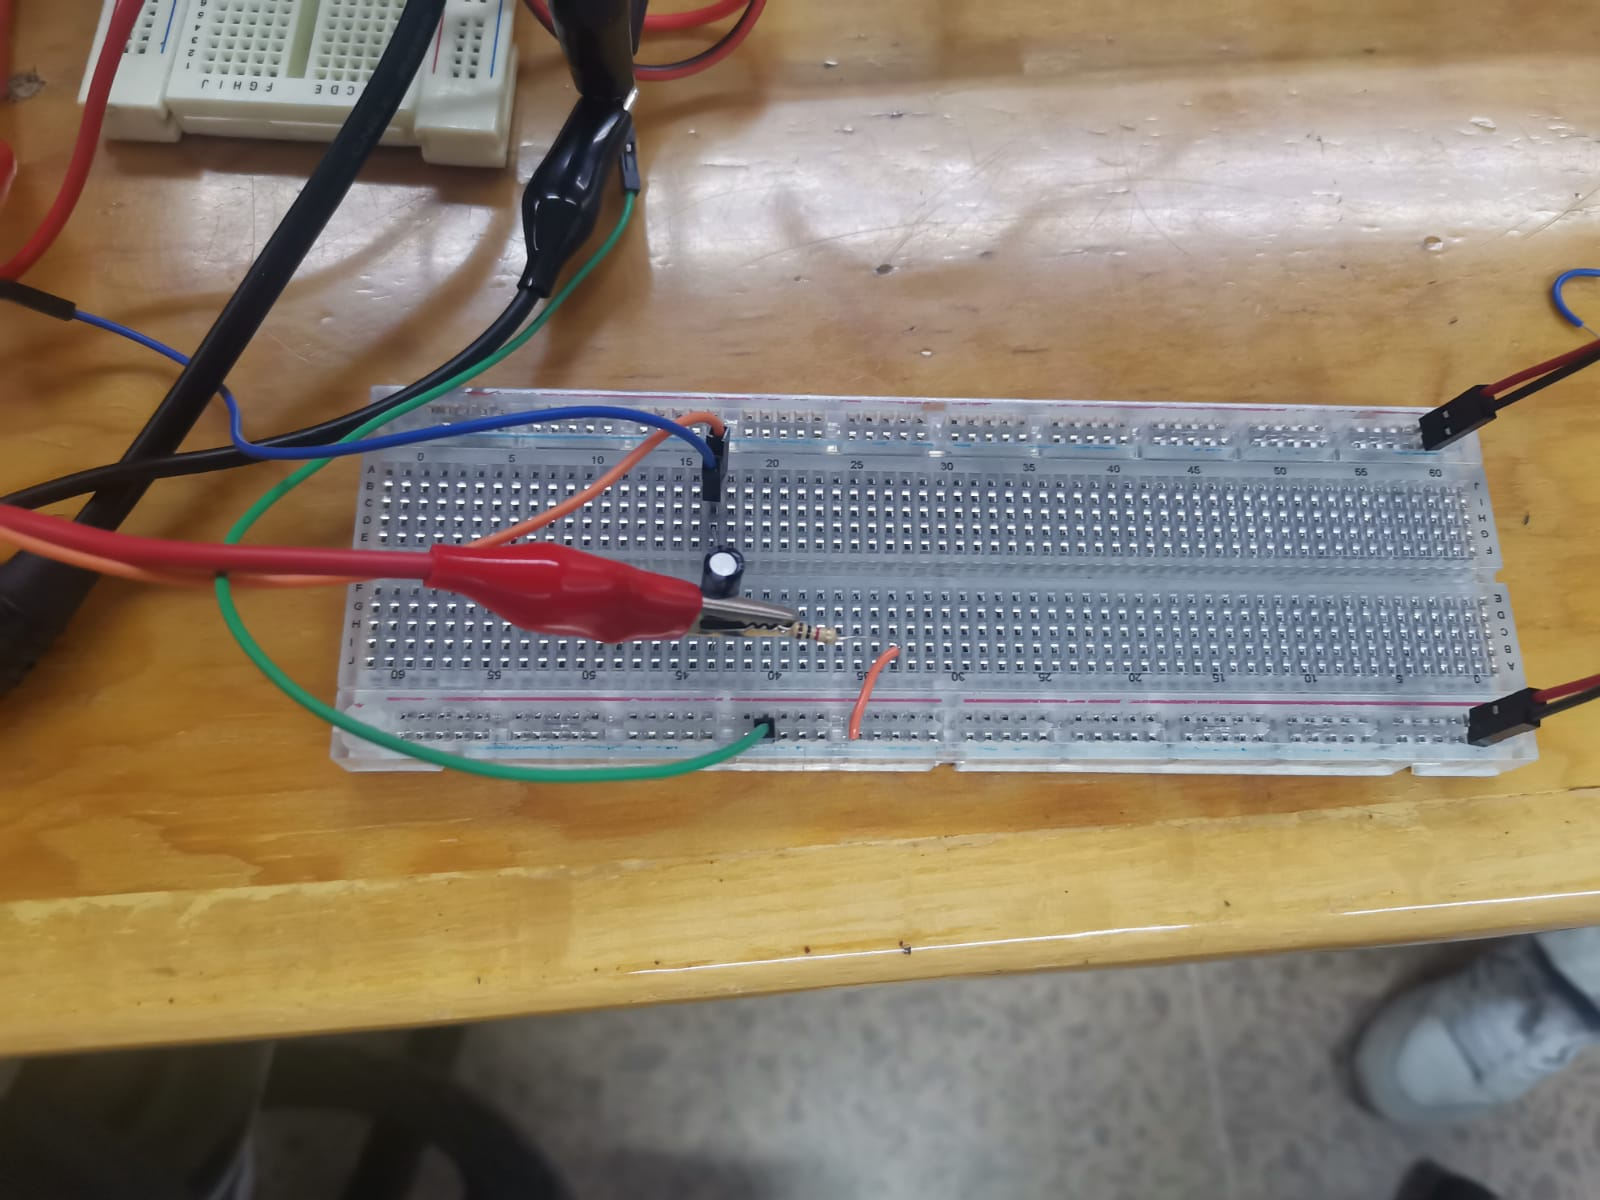
\includegraphics[width=\textwidth]{circuitoRC.jpeg}
					\caption{Circuito RC realizado en laboratorio}
				\end{subfigure}
				\hspace{0.08\textwidth}
				\begin{subfigure}{0.45\textwidth}
					\centering
					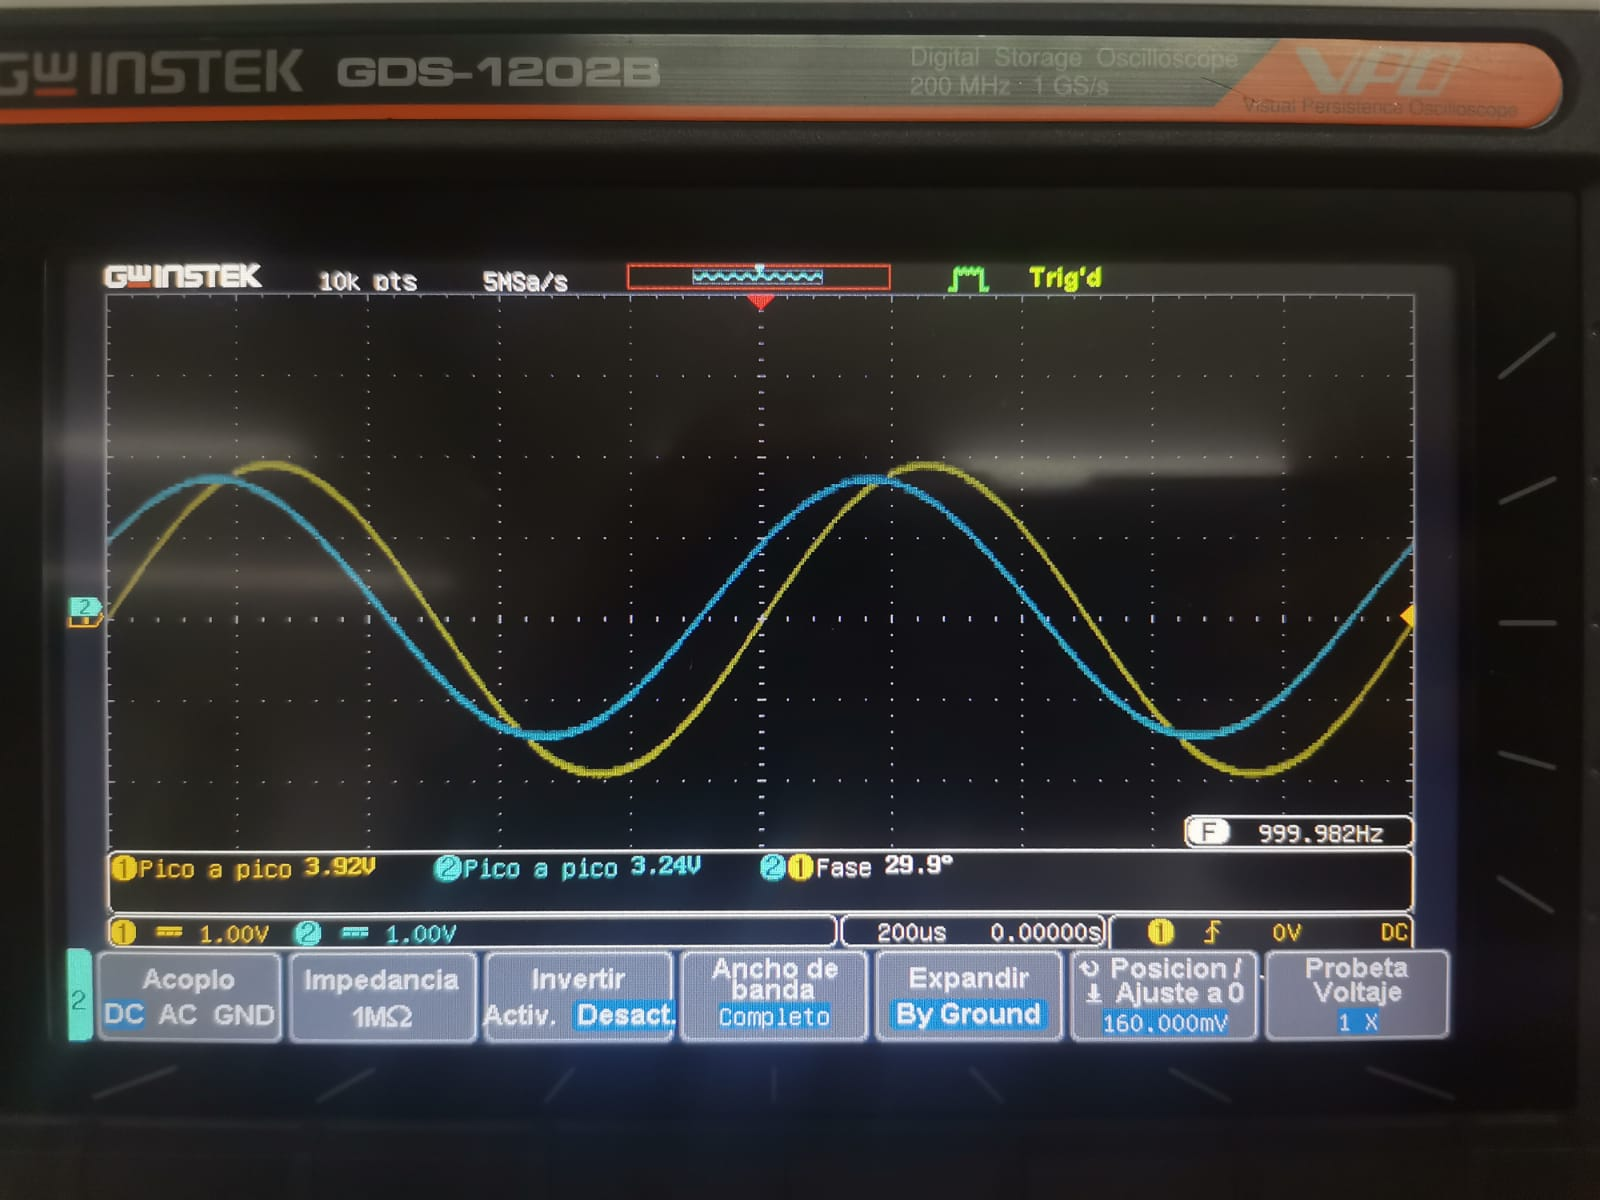
\includegraphics[width=\textwidth]{circuitoRC_grafica.jpeg}
					\caption{Oscilograma del circuito RC}
				\end{subfigure}
			\end{figure}
	
			\begin{center}
				\begin{circuitikz} \draw
					(0,0) to[sV, l=$V_f$, invert] (0,3) 
					to[C=220 nF] (3,3)       
					to[R=1K$\Omega$] (3,0)   
					-- (0,0);                         
				\end{circuitikz} 
			\end{center}
			
			\hspace{0.5cm}Esta es una representación del circuito armado en laboratorio, en el podemos ver que se utilizó una resistencia de $R=1$[K$\Omega$] y un capacitor de $C=220$[nF].
			Para la señal sinusoidal de entrada se ingresaron los valores de: frecuencia de $f = 1$[KHz] y amplitud $A=4$[Vpp]
\newpage
		\subsubsection{Parte teórica}
			
			\hspace{0.5cm}Un circuito RC está conformado por una resistencia y un capacitor conectados en serie o en paralelo. En este caso, se tiene un circuito RC en serie alimentado con una señal senoidal.
			
			\hspace{0.5cm}El comportamiento del circuito depende de la frecuencia de la señal de entrada, ya que el capacitor presenta una oposición al paso de la corriente conocida como reactancia capacitiva, la cual está dada por:
			
			\[
			X_C = \frac{1}{2\pi f C}
			\]
			
			Donde:
			\begin{itemize}
				\item $X_C$ es la reactancia capacitiva [$\Omega$]
				\item $f$ es la frecuencia [Hz]
				\item $C$ es la capacitancia [F]
			\end{itemize}
			
			\hspace{0.5cm}Para una señal senoidal, el circuito RC actúa como un filtro, cuyo comportamiento depende del punto de salida. Si la salida se toma en el capacitor, el circuito funciona como un filtro pasa-bajas; si se toma en la resistencia, funciona como un filtro pasa-altas.
			
			\hspace{0.5cm}La relación entre el voltaje de salida y el voltaje de entrada está dada por la función de transferencia del circuito. Para el caso de salida en el capacitor:
			
			\[
			H(j\omega) = \frac{1}{1 + j\omega RC}
			\]
			
			Y para la salida en la resistencia:
			
			\[
			H(j\omega) = \frac{j\omega RC}{1 + j\omega RC}
			\]
			
			Donde $\omega = 2\pi f$ es la frecuencia angular.
			
			Además, un parámetro importante es la constante de tiempo del circuito, definida como:
			
			\[
			\tau = RC
			\]
			
			Esta constante determina la rapidez con la que el capacitor se carga y descarga.
			
			Para los valores utilizados en la práctica:
			
			\[
			R = 1\,k\Omega = 1000\,\Omega
			\]
			\[
			C = 220\,nF = 220 \times 10^{-9}\,F
			\]
			
			La constante de tiempo es:
			
			\[
			\tau = (1000)(220 \times 10^{-9}) = 2.2 \times 10^{-4}\,s = 220\,\mu s
			\]
			
			Por otro lado, la frecuencia de corte del circuito se define como:
			
			\[
			f_c = \frac{1}{2\pi RC}
			\]
			
			Sustituyendo valores:
			
			\[
			f_c = \frac{1}{2\pi (1000)(220 \times 10^{-9})} \approx 723\,Hz
			\]
			
			\hspace{0.5cm}El circuito RC presenta un comportamiento dependiente de la frecuencia, permitiendo analizar fenómenos de filtrado y desfase entre voltaje y corriente.
		
		\subsubsection{Análisis senoidal permanente (Excitación senoidal)}
		
			Para el circuito RC, aplicando la Ley de Voltajes de Kirchhoff:
			
			\[
			v_f(t) = v_R(t) + v_C(t)
			\]
			
			Sabemos que:
			
			\[
			v_R(t) = Ri(t), \quad i(t) = C \frac{dv_C(t)}{dt}
			\]
			
			Sustituyendo:
			
			\[
			v_f(t) = RC \frac{dv_C(t)}{dt} + v_C(t)
			\]
			
			Esta es la ecuación diferencial del circuito.
			
			\textbf{Parámetros:}
			
			\[
			R = 1000 \ \Omega, \quad C = 220 \times 10^{-9} F
			\]
			
			\[
			\tau = RC = 220 \ \mu s
			\]
			
			\textbf{Frecuencia 1 kHz:}
			
			Para una frecuencia de $f = 1000$ Hz, primero se calcula la frecuencia angular:
			
			\[
			\omega = 2\pi f = 2\pi(1000) = 2000\pi \ \text{rad/s}
			\]
			
			Sustituyendo en la expresión de la reactancia capacitiva:
			
			\[
			X_C = \frac{1}{\omega C} = \frac{1}{(2000\pi)(220 \times 10^{-9})}
			\]
			
			\[
			X_C \approx 723 \ \Omega
			\]
			
			La impedancia del circuito RC en forma compleja es:
			
			\[
			Z = R - jX_C = 1000 - j723
			\]
			
			Su magnitud es:
			
			\[
			|Z| = \sqrt{R^2 + X_C^2} = \sqrt{(1000)^2 + (723)^2}
			\]
			
			\[
			|Z| \approx 1234 \ \Omega
			\]
			
			El ángulo de fase es:
			
			\[
			\theta = -\tan^{-1}\left(\frac{X_C}{R}\right) = -\tan^{-1}\left(\frac{723}{1000}\right)
			\]
			
			\[
			\theta \approx -35.85^\circ
			\]
			
			Por lo tanto, la impedancia en forma polar es:
			
			\[
			Z \approx 1234 \angle -35.85^\circ \ \Omega
			\]
			
			\vspace{0.5cm}
			
			\begin{figure}[H]
				\centering
				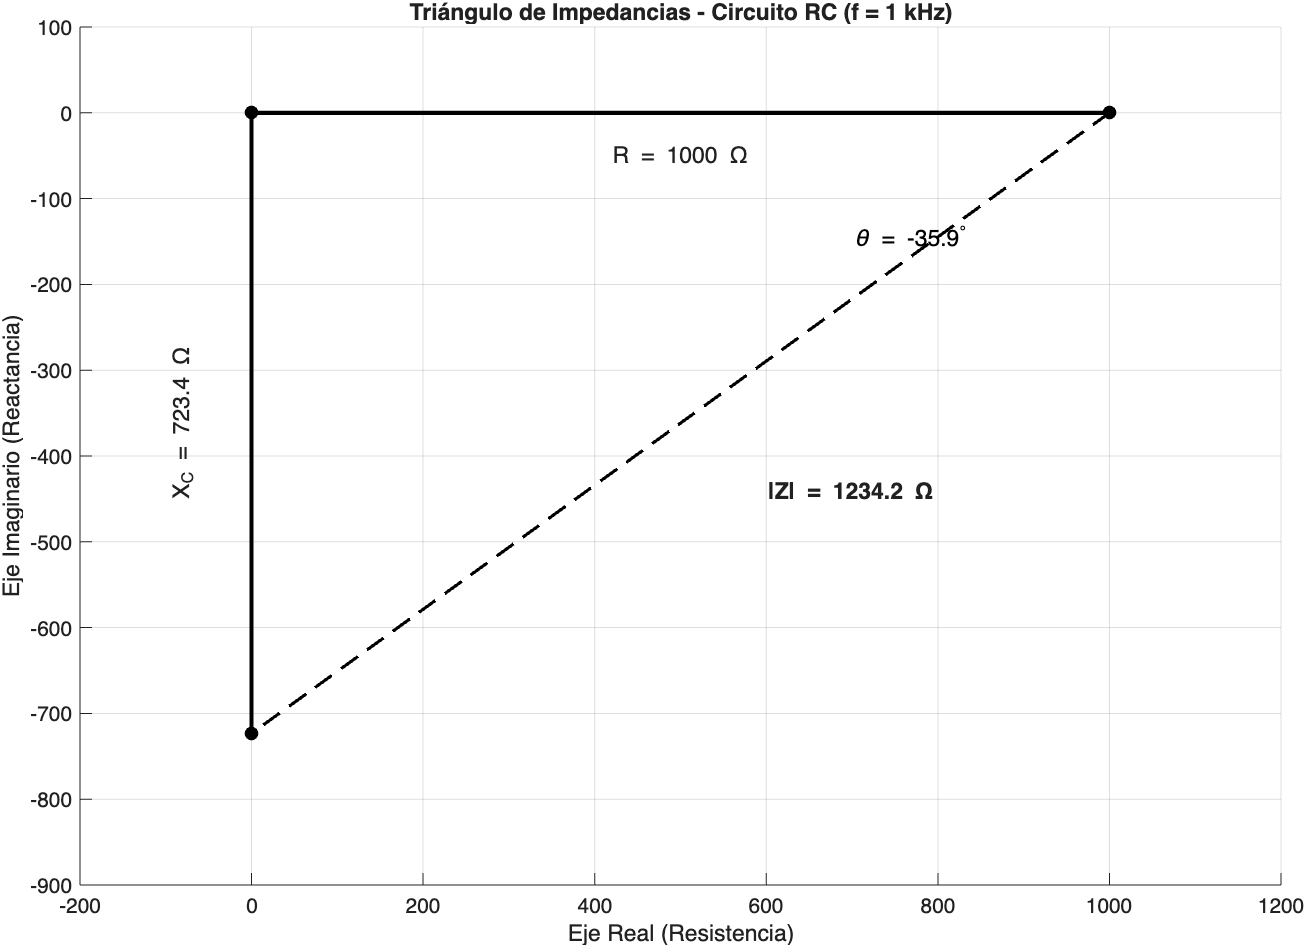
\includegraphics[width=0.75\linewidth]{trianguloImpRC1.png}
				\caption{Triangulo de impedancias del circuito RC con una frecuencia de 1kHz.}
			\end{figure}
			
			\begin{figure}[H]
				\centering
				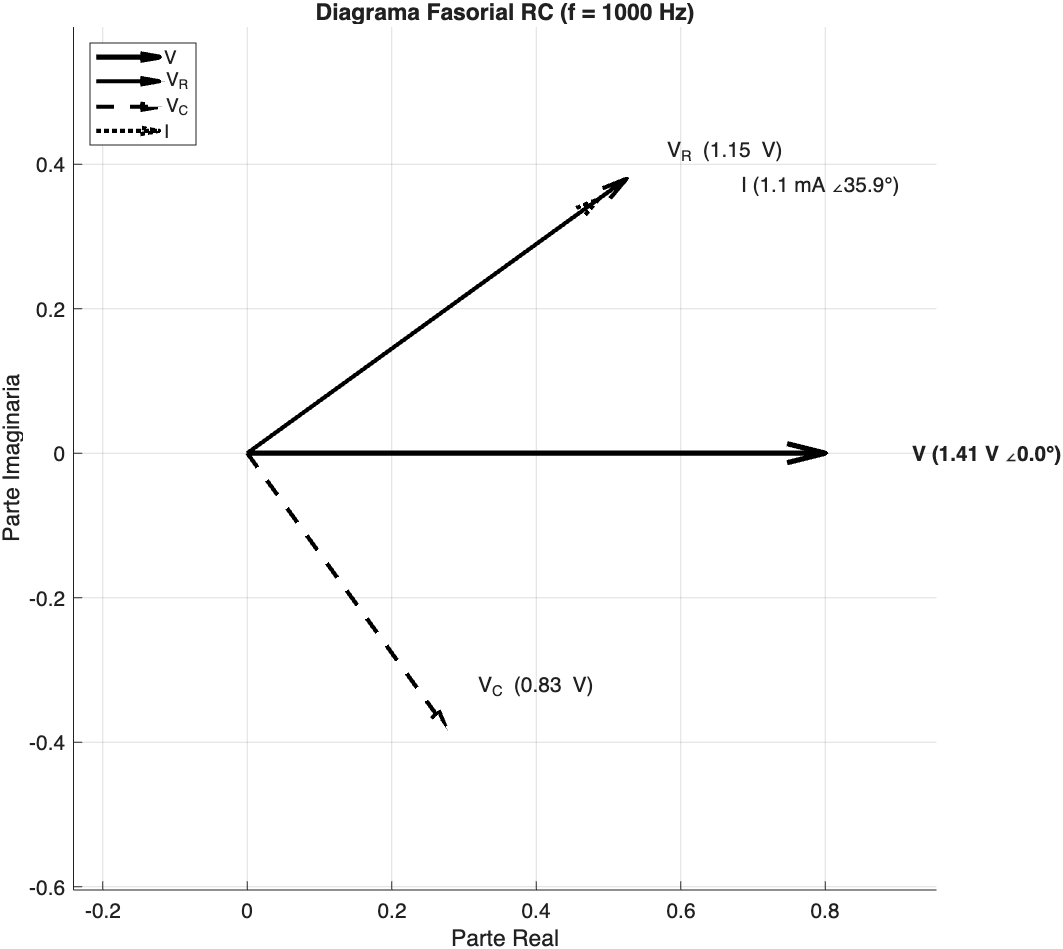
\includegraphics[width=0.75\linewidth]{fasor1.png}
				\caption{Diagrama fasorial de un circuito RC con una frecuencia de 1kHz.}
			\end{figure}
			
			\textbf{Frecuencia 2 kHz:}
			
			Para $f = 2000$ Hz:
			
			\[
			\omega = 2\pi(2000) = 4000\pi \ \text{rad/s}
			\]
			
			Reactancia capacitiva:
			
			\[
			X_C = \frac{1}{\omega C} = \frac{1}{(4000\pi)(220 \times 10^{-9})}
			\]
			
			\[
			X_C \approx 361.7 \ \Omega
			\]
			
			Impedancia en forma compleja:
			
			\[
			Z = 1000 - j361.7
			\]
			
			Magnitud:
			
			\[
			|Z| = \sqrt{(1000)^2 + (361.7)^2}
			\]
			
			\[
			|Z| \approx 1063 \ \Omega
			\]
			
			Ángulo de fase:
			
			\[
			\theta = -\tan^{-1}\left(\frac{361.7}{1000}\right)
			\]
			
			\[
			\theta \approx -19.88^\circ
			\]
			
			Forma polar:
			
			\[
			Z \approx 1063 \angle -19.88^\circ \ \Omega
			\]
			
			\begin{figure}[H]
				\centering
				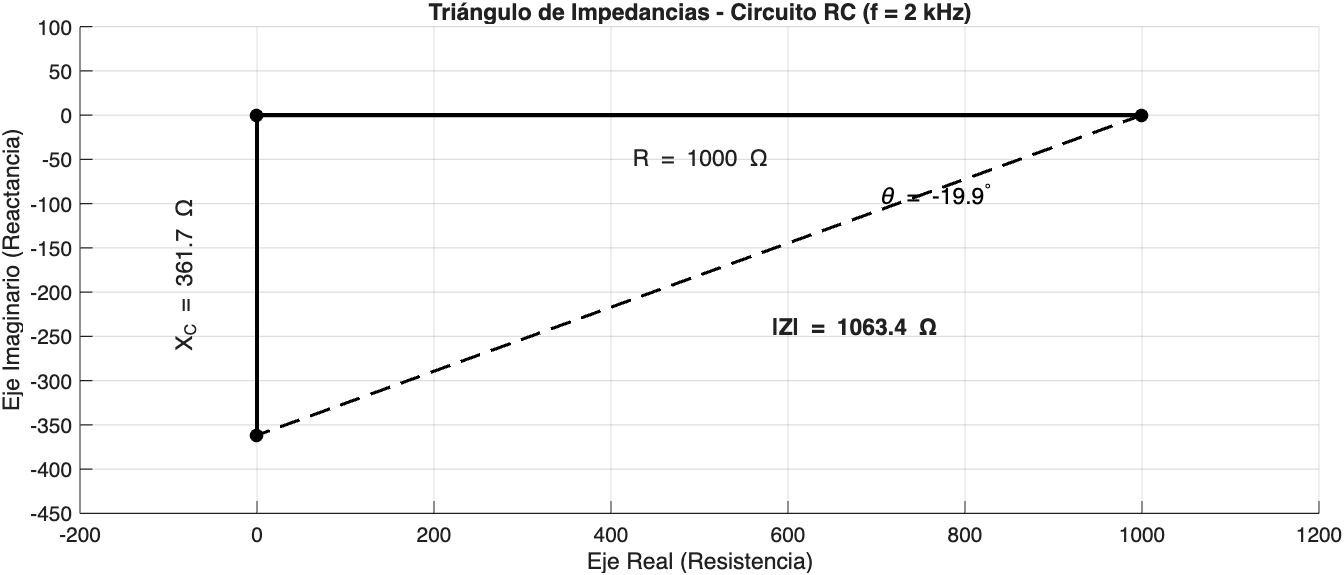
\includegraphics[width=0.85\linewidth]{trianguloRC2.png}
				\caption{Triangulo de impedancias del circuito RC con una frecuencia de 2kHz.}
			\end{figure}
			
			\begin{figure}[H]
				\centering
				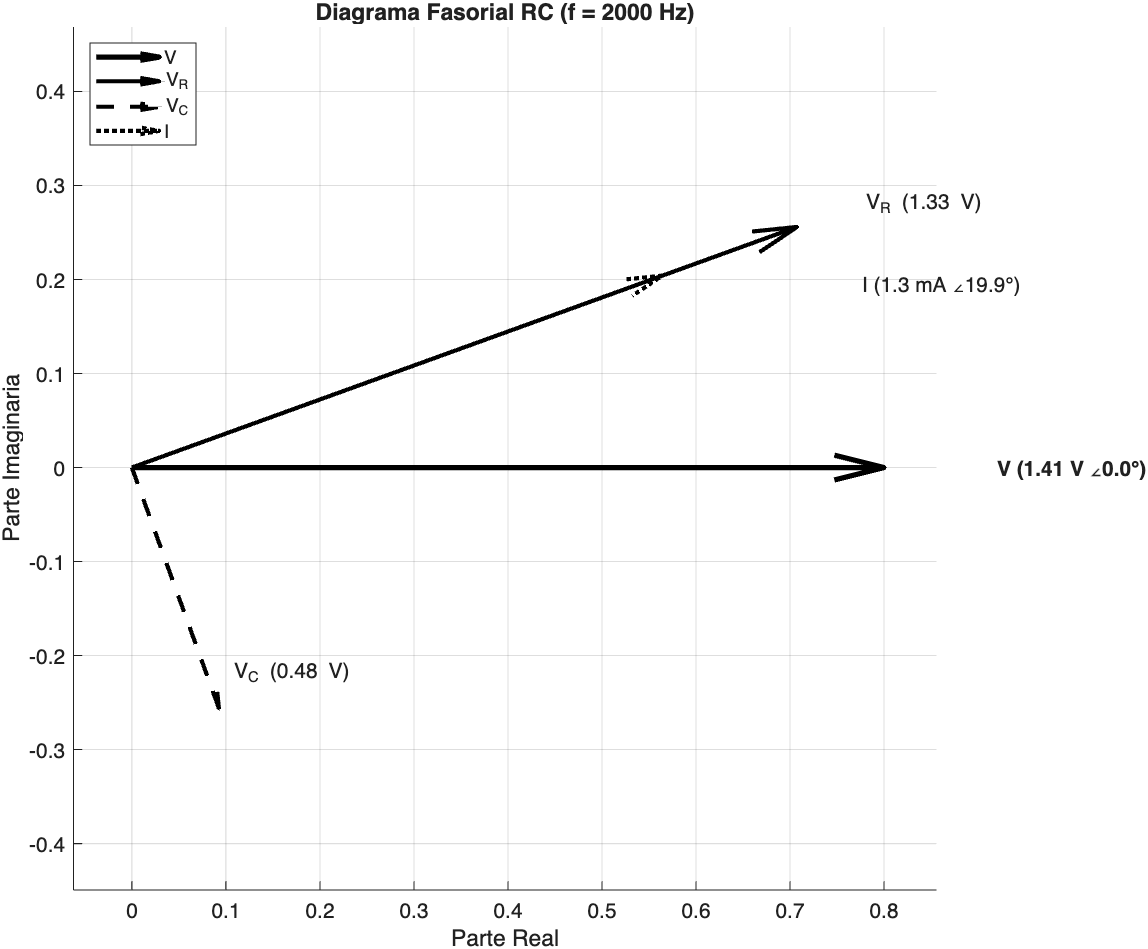
\includegraphics[width=0.75\linewidth]{fasor2.png}
				\caption{Diagrama fasorial de un circuito RC con una frecuencia de 2kHz.}
			\end{figure}
			
			Se observa que al aumentar la frecuencia, disminuye la reactancia capacitiva, reduciendo el desfase.
	
	\subsection{Circuito RL}
	
		\subsubsection{Parte experimental}
		
			\begin{figure}[H]
				\centering
				\begin{subfigure}{0.45\textwidth}
					\centering
					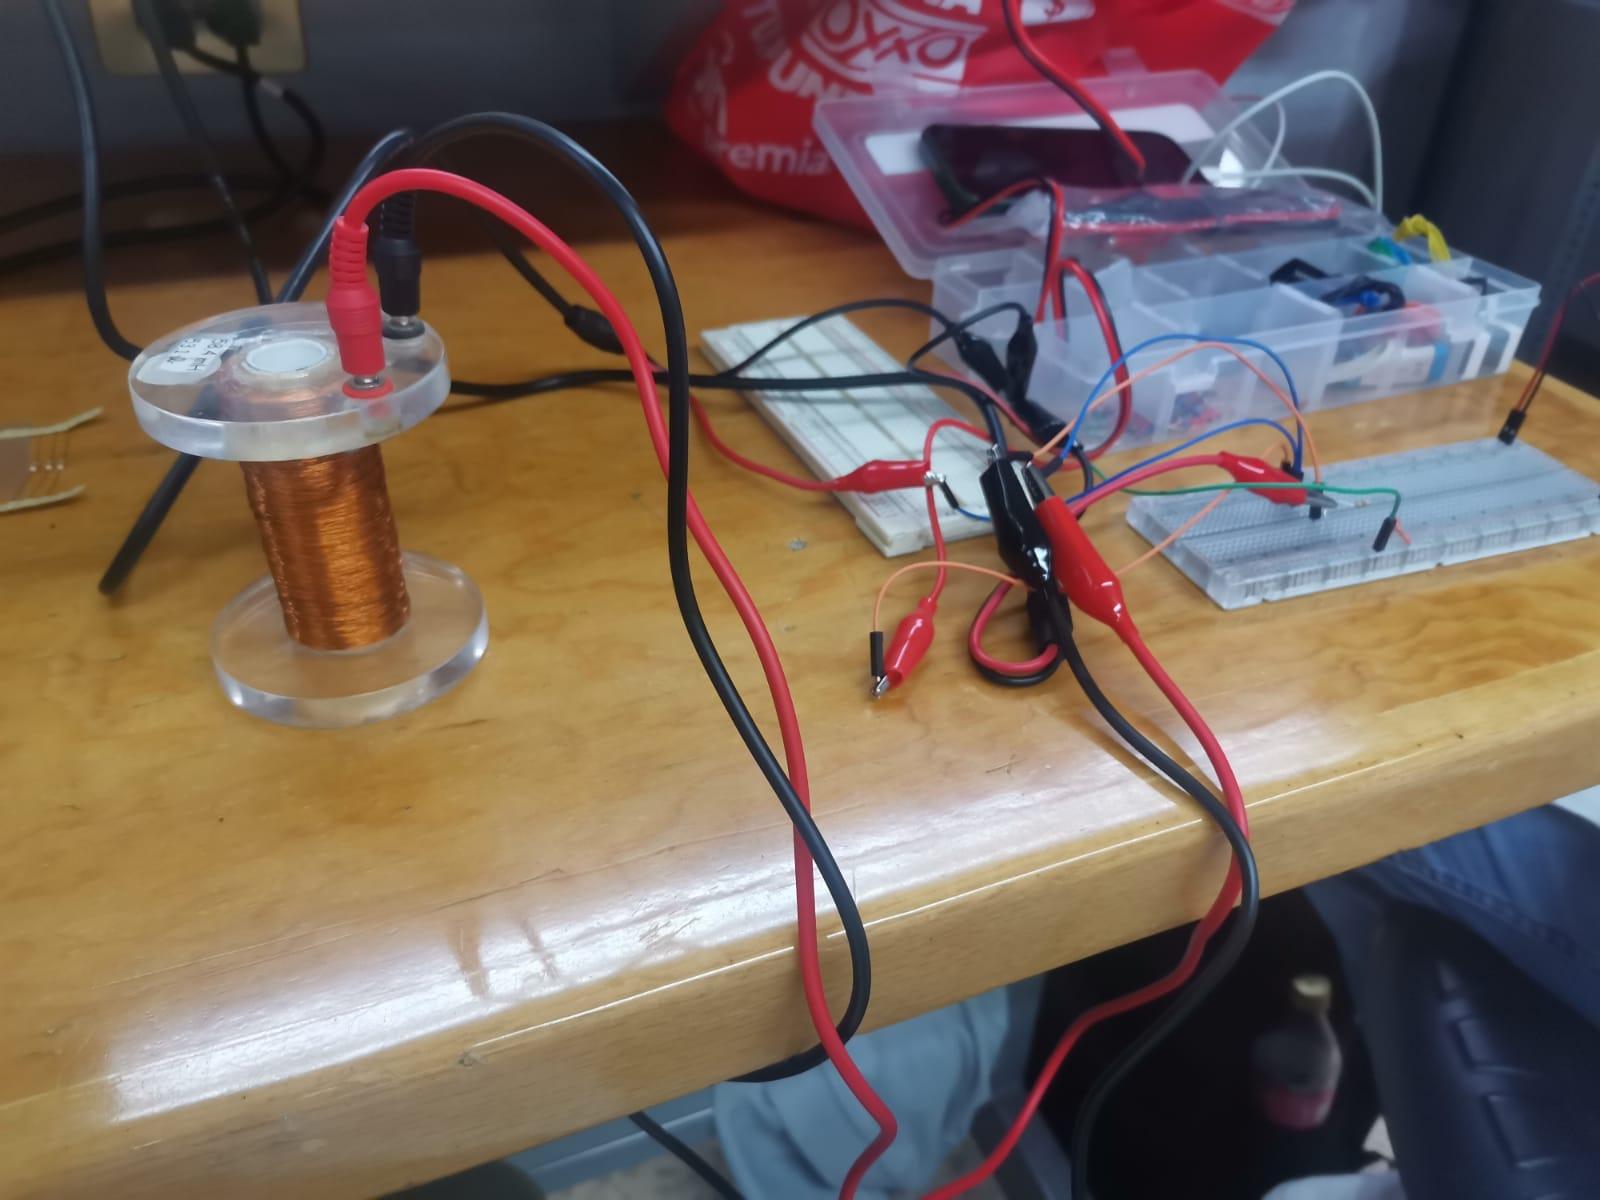
\includegraphics[width=\textwidth]{circuitoRL.jpeg}
					\caption{Circuito RL realizado en laboratorio}
				\end{subfigure}
				\hspace{0.08\textwidth}
				\begin{subfigure}{0.45\textwidth}
					\centering
					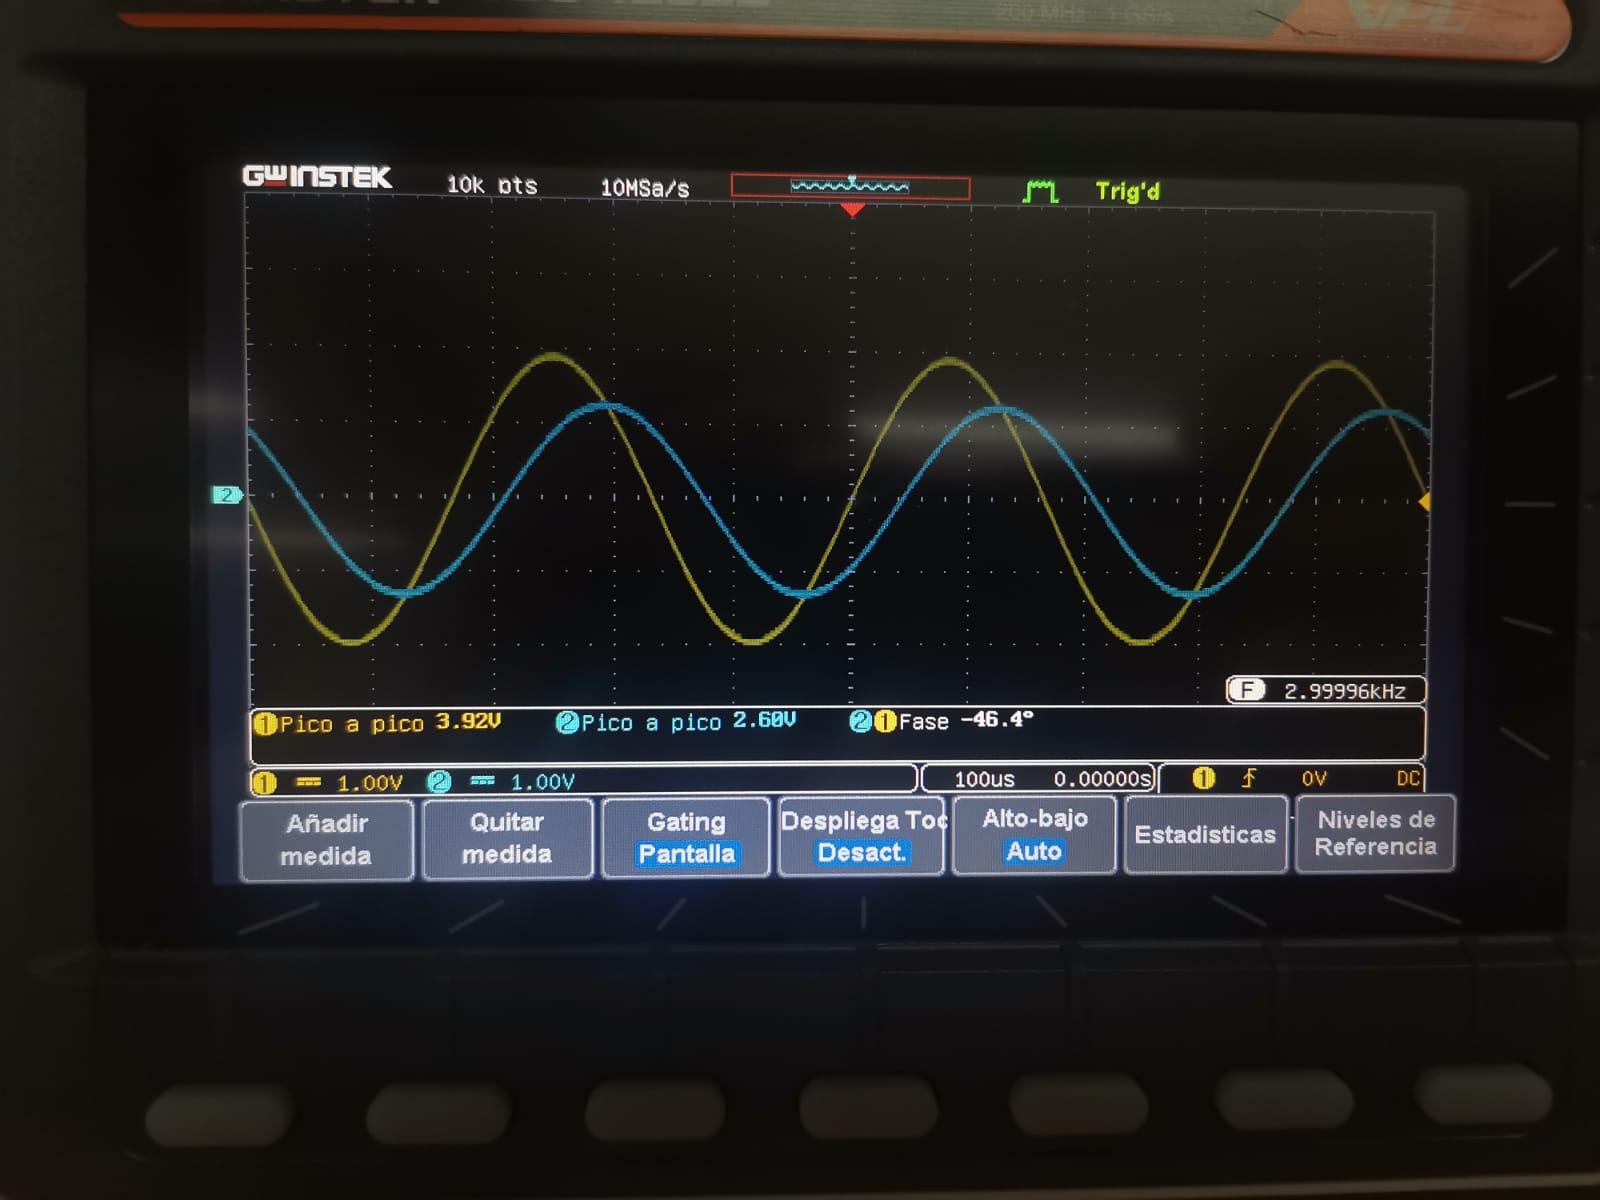
\includegraphics[width=\textwidth]{circuitoRL_graficas.jpeg}
					\caption{Oscilograma del circuito RL}
				\end{subfigure}
			\end{figure}
		
			\begin{center}
				\begin{circuitikz} \draw
					(0,0) to[sV, l=$V_f$, invert] (0,3) 
					to[L=61.8 mH] (3,3)       
					to[R=1K$\Omega$] (3,0)   
					-- (0,0);                         
				\end{circuitikz} 
			\end{center}
	
		\subsubsection{Parte teórica}
			
			\hspace{0.5cm}Un circuito RL está conformado por una resistencia y un inductor conectados en serie o en paralelo. En este caso, se analiza un circuito RL en serie alimentado por una señal senoidal.
			
			\hspace{0.5cm}El comportamiento del circuito depende de la frecuencia de la señal de entrada, ya que el inductor presenta una oposición al paso de la corriente conocida como reactancia inductiva, la cual está dada por:
			
			\[
			X_L = \omega L = 2\pi f L
			\]
			
			Donde:
			\begin{itemize}
				\item $X_L$ es la reactancia inductiva [$\Omega$]
				\item $f$ es la frecuencia [Hz]
				\item $L$ es la inductancia [H]
			\end{itemize}
			
			\hspace{0.5cm}Para una señal senoidal, el circuito RL también presenta un comportamiento de filtrado. Si la salida se toma en la resistencia, el circuito actúa como un filtro pasa-bajas; mientras que si se toma en el inductor, se comporta como un filtro pasa-altas.
			
			\hspace{0.5cm}La relación entre el voltaje de salida y el voltaje de entrada se puede expresar mediante la función de transferencia. Para el caso de salida en la resistencia:
			
			\[
			H(j\omega) = \frac{R}{R + j\omega L}
			\]
			
			Y para la salida en el inductor:
			
			\[
			H(j\omega) = \frac{j\omega L}{R + j\omega L}
			\]
			
			Donde $\omega = 2\pi f$ es la frecuencia angular.
			
			La impedancia total del circuito RL en forma compleja es:
			
			\[
			Z = R + jX_L
			\]
			
			Su magnitud está dada por:
			
			\[
			|Z| = \sqrt{R^2 + X_L^2}
			\]
			
			Y el ángulo de fase es:
			
			\[
			\theta = \tan^{-1}\left(\frac{X_L}{R}\right)
			\]
			
			Este ángulo indica que la corriente se encuentra retrasada respecto al voltaje en un circuito RL.
			
			Además, un parámetro importante es la constante de tiempo del circuito, definida como:
			
			\[
			\tau = \frac{L}{R}
			\]
			
			La cual determina la rapidez con la que la corriente alcanza su valor estable.
			
			Para los valores utilizados en la práctica:
			
			\[
			R = 1\,k\Omega = 1000\,\Omega
			\]
			
			\[
			L = 61.8\,mH = 61.8 \times 10^{-3}\,H
			\]
			
			La constante de tiempo es:
			
			\[
			\tau = \frac{61.8 \times 10^{-3}}{1000} = 6.18 \times 10^{-5}\,s = 61.8\,\mu s
			\]
			
			Por otro lado, la frecuencia de corte del circuito está dada por:
			
			\[
			f_c = \frac{R}{2\pi L}
			\]
			
			Sustituyendo valores:
			
			\[
			f_c = \frac{1000}{2\pi (61.8 \times 10^{-3})} \approx 2575\,Hz
			\]
			
			Esta frecuencia representa el punto en el cual la respuesta del circuito comienza a cambiar significativamente.
			
			\hspace{0.5cm}En conclusión, el circuito RL presenta un comportamiento dependiente de la frecuencia, en el cual la reactancia inductiva aumenta conforme incrementa la frecuencia, provocando un mayor desfase entre el voltaje y la corriente, así como un comportamiento característico de filtrado.
		
		\subsubsection{Análisis senoidal permanente (Excitación senoidal)}
		
			Para el circuito RL, aplicando la Ley de Voltajes de Kirchhoff:
			
			\[
			v_f(t) = v_R(t) + v_L(t)
			\]
			
			Sabemos que:
			
			\[
			v_R(t) = Ri(t), \quad v_L(t) = L \frac{di(t)}{dt}
			\]
			
			Sustituyendo:
			
			\[
			v_f(t) = L \frac{di(t)}{dt} + Ri(t)
			\]
			
			En régimen senoidal permanente, se trabaja en el dominio fasorial, donde la impedancia del circuito es:
			
			\[
			Z = R + j\omega L
			\]
			
			\textbf{Parámetros del circuito:}
			
			\[
			R = 1000 \ \Omega, \quad L = 61.8 \times 10^{-3} \ H
			\]
			
			\vspace{0.3cm}
			
			\textbf{Frecuencia 1 kHz:}
			
			Para una frecuencia de $f = 1000$ Hz, se calcula primero la frecuencia angular:
			
			\[
			\omega = 2\pi f = 2\pi(1000) = 2000\pi \ \text{rad/s}
			\]
			
			Sustituyendo en la expresión de la reactancia inductiva:
			
			\[
			X_L = \omega L = (2000\pi)(61.8 \times 10^{-3})
			\]
			
			\[
			X_L \approx 388.4 \ \Omega
			\]
			
			La impedancia del circuito RL en forma compleja es:
			
			\[
			Z = R + jX_L = 1000 + j388.4
			\]
			
			Su magnitud se obtiene como:
			
			\[
			|Z| = \sqrt{R^2 + X_L^2} = \sqrt{(1000)^2 + (388.4)^2}
			\]
			
			\[
			|Z| \approx 1073 \ \Omega
			\]
			
			El ángulo de fase está dado por:
			
			\[
			\theta = \tan^{-1}\left(\frac{X_L}{R}\right) = \tan^{-1}\left(\frac{388.4}{1000}\right)
			\]
			
			\[
			\theta \approx 21.2^\circ
			\]
			
			Por lo tanto, la impedancia en forma polar es:
			
			\[
			Z \approx 1073 \angle 21.2^\circ \ \Omega
			\]
			
			\begin{figure}[H]
				\centering
				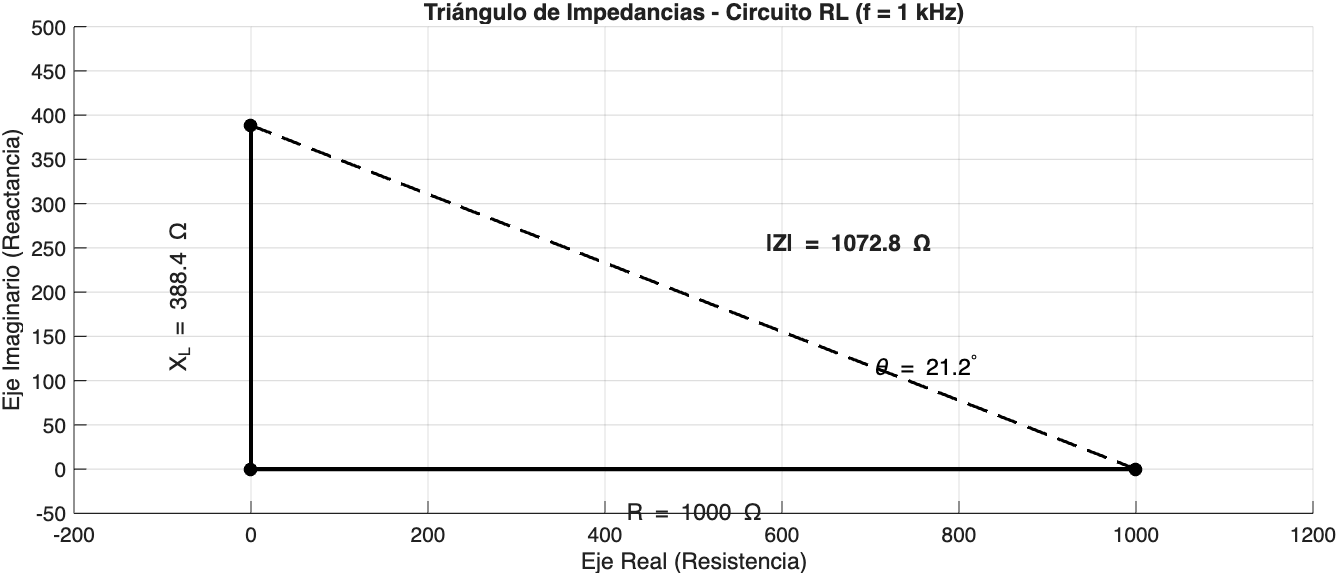
\includegraphics[width=0.85\linewidth]{trianguloRL1.png}
				\caption{Triangulo de impedancias del circuito RL con una frecuencia de 1kHz.}
			\end{figure}
			
			\begin{figure}[H]
				\centering
				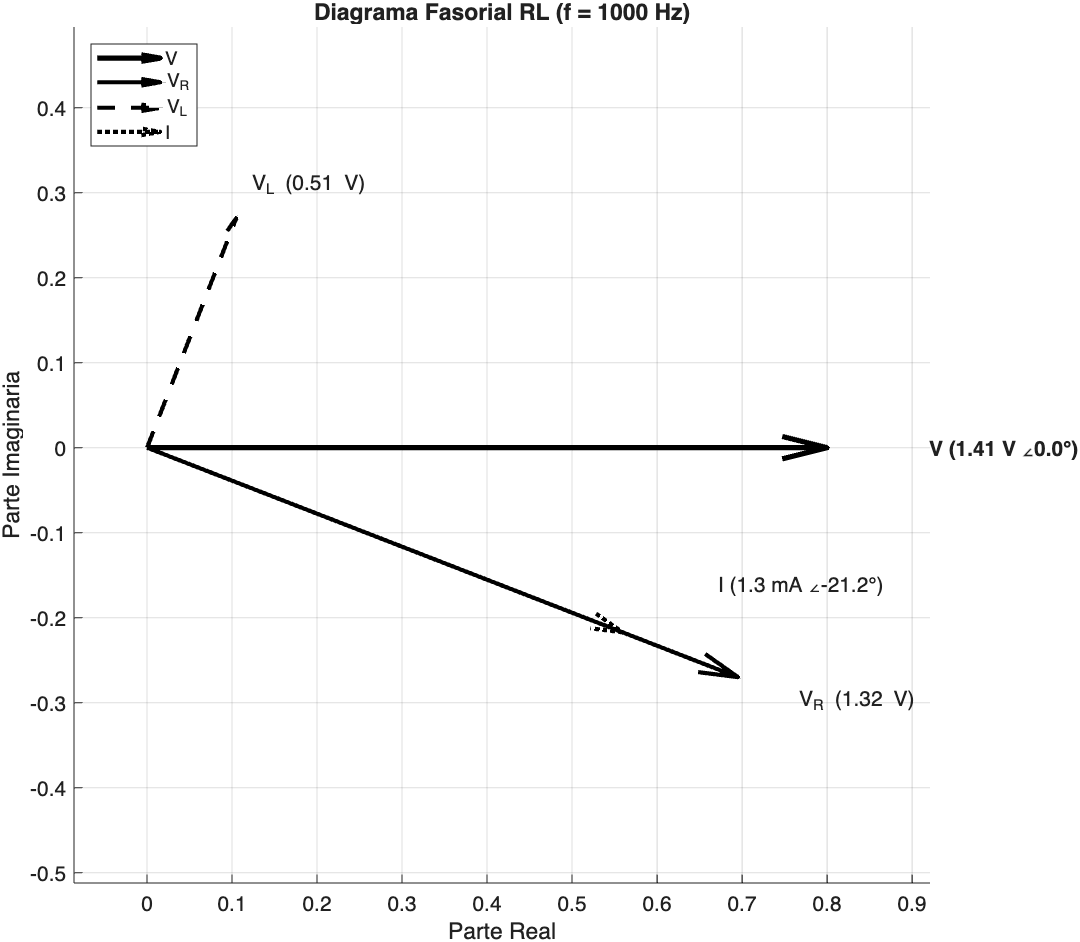
\includegraphics[width=0.75\linewidth]{fasorL1.png}
				\caption{Diagrama fasorial de un circuito RL con una frecuencia de 1kHz.}
			\end{figure}
			
			\vspace{0.5cm}
			
			\textbf{Frecuencia 2 kHz:}
			
			Para $f = 2000$ Hz:
			
			\[
			\omega = 2\pi(2000) = 4000\pi \ \text{rad/s}
			\]
			
			Reactancia inductiva:
			
			\[
			X_L = \omega L = (4000\pi)(61.8 \times 10^{-3})
			\]
			
			\[
			X_L \approx 776.8 \ \Omega
			\]
			
			Impedancia en forma compleja:
			
			\[
			Z = 1000 + j776.8
			\]
			
			Magnitud:
			
			\[
			|Z| = \sqrt{(1000)^2 + (776.8)^2}
			\]
			
			\[
			|Z| \approx 1265 \ \Omega
			\]
			
			Ángulo de fase:
			
			\[
			\theta = \tan^{-1}\left(\frac{776.8}{1000}\right)
			\]
			
			\[
			\theta \approx 37.8^\circ
			\]
			
			Forma polar:
			
			\[
			Z \approx 1265 \angle 37.8^\circ \ \Omega
			\]
			
			\begin{figure}[H]
				\centering
				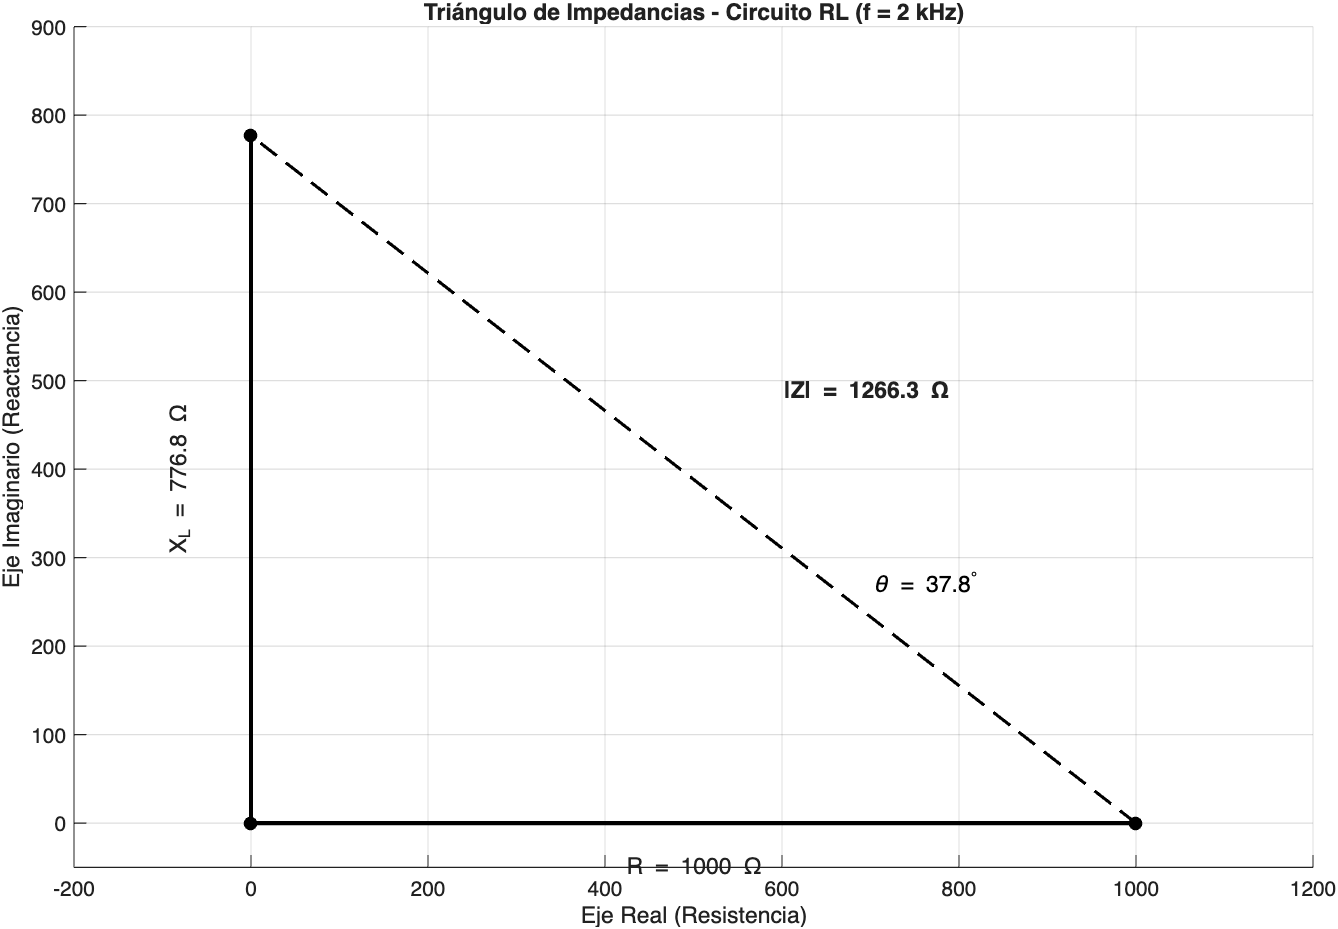
\includegraphics[width=0.65\linewidth]{trianguloRL2.png}
				\caption{Triangulo de impedancias del circuito RL con una frecuencia de 2kHz.}
			\end{figure}
			
			\begin{figure}[H]
				\centering
				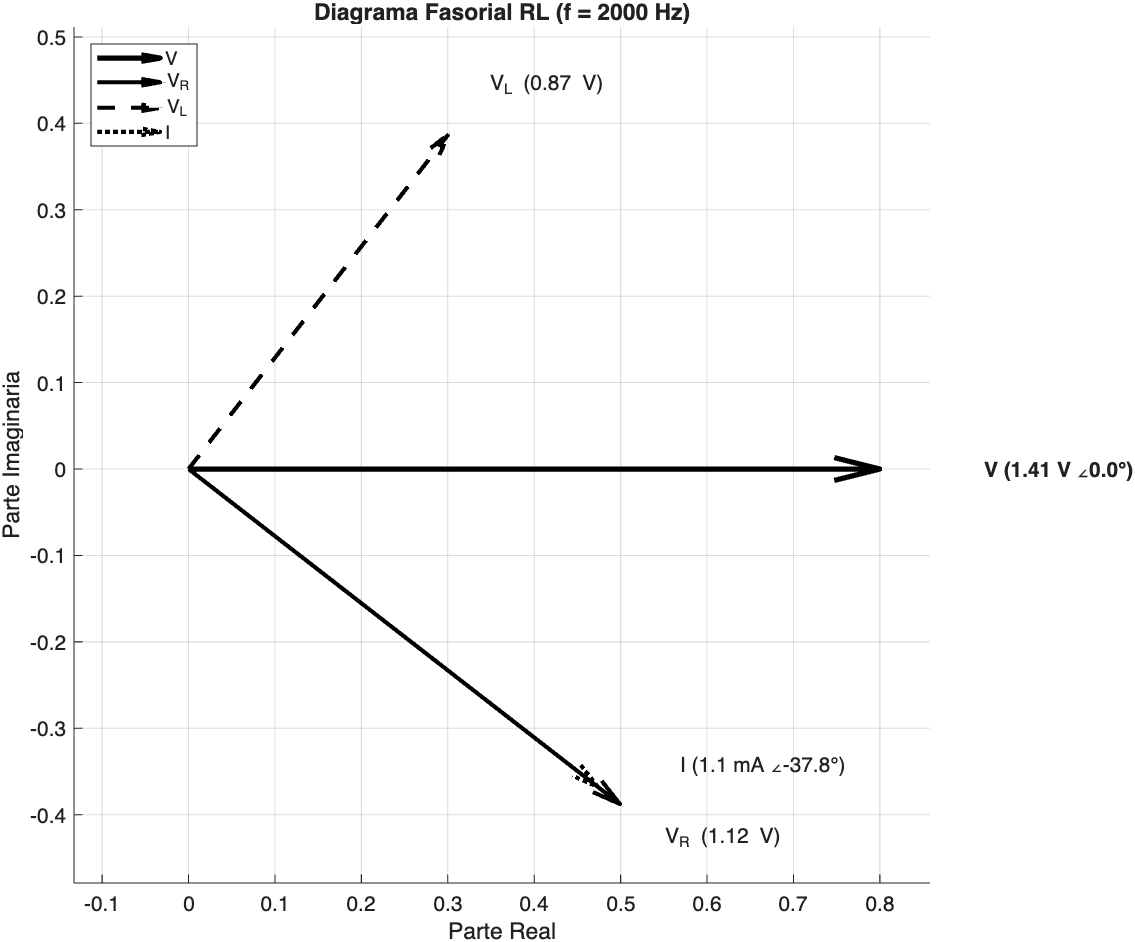
\includegraphics[width=0.65\linewidth]{fasorL2.png}
				\caption{Diagrama fasorial de un circuito RL con una frecuencia de 2kHz.}
			\end{figure}
			
			\textbf{Interpretación:}
			
			\hspace{0.5cm}Se observa que al aumentar la frecuencia, la reactancia inductiva incrementa, lo que provoca un aumento en la impedancia total y un mayor ángulo de desfase. Esto indica que la corriente se retrasa más respecto al voltaje conforme aumenta la frecuencia.
			
	\subsection{Análisis de respuesta transitoria y permanente (Excitación en DC)}
	
		\subsubsection{Circuito RC}
		
			Para el circuito RC, aplicando la Ley de Voltajes de Kirchhoff:
			
			\[
			v_f(t) = v_R(t) + v_C(t)
			\]
			
			Sabemos que:
			
			\[
			v_R(t) = Ri(t), \quad i(t) = C \frac{dv_C(t)}{dt}
			\]
			
			Sustituyendo:
			
			\[
			v_f(t) = RC \frac{dv_C(t)}{dt} + v_C(t)
			\]
			
			Esta es la ecuación diferencial del circuito.
			
			\vspace{0.3cm}
			
			\textbf{Solución de la ecuación diferencial}
			
			Para una entrada de voltaje constante $V$, la solución es:
			
			\[
			v_C(t) = V\left(1 - e^{-t/RC}\right)
			\]
			
			Sustituyendo valores:
			
			\[
			R = 1000 \ \Omega, \quad C = 220 \times 10^{-9} \ F
			\]
			
			\[
			\tau = RC = 2.2 \times 10^{-4} \ s
			\]
			
			\[
			v_C(t) = V\left(1 - e^{-t/0.00022}\right)
			\]
			
			El voltaje en la resistencia es:
			
			\[
			v_R(t) = V e^{-t/RC}
			\]
			
			\[
			v_R(t) = V e^{-t/0.00022}
			\]
			
			La corriente en el circuito:
			
			\[
			i(t) = \frac{V}{R} e^{-t/RC}
			\]
			
			\vspace{0.3cm}
			
			\textbf{Comportamiento}
			
			\begin{itemize}
				\item En $t = 0$, el capacitor se comporta como un cortocircuito.
				\item La corriente es máxima al inicio.
				\item El capacitor se carga exponencialmente.
				\item En estado permanente ($t \to \infty$), el capacitor se comporta como circuito abierto.
				\item El voltaje final en el capacitor es igual al de la fuente.
			\end{itemize}
			
			\begin{figure}[H]
				\centering
				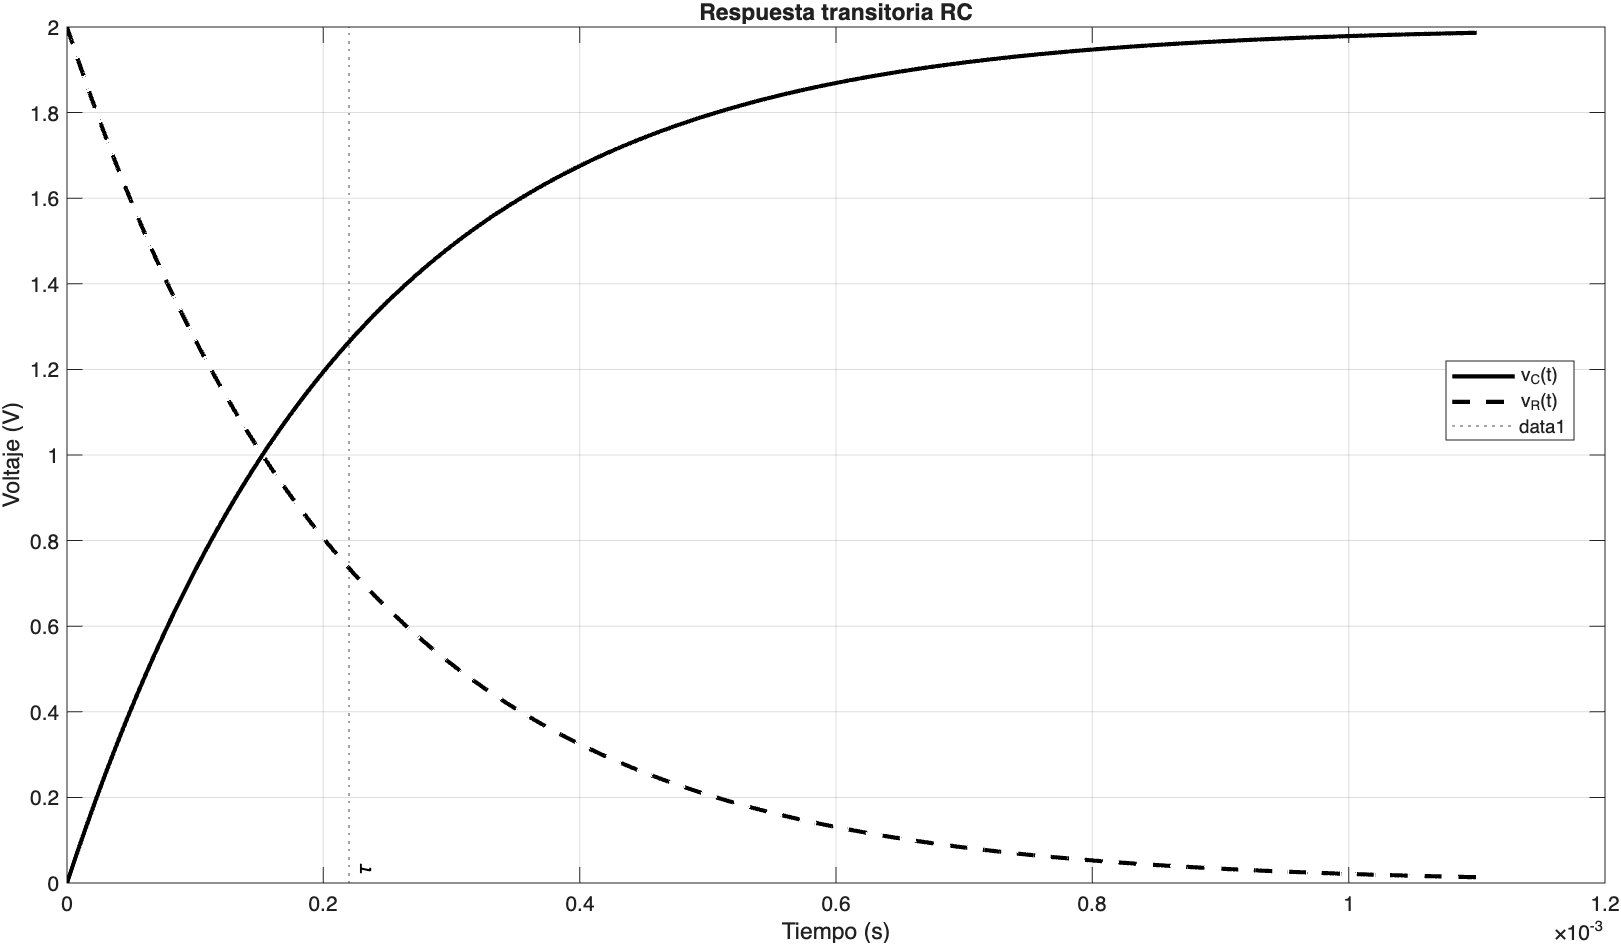
\includegraphics[width=0.75\linewidth]{transitoriaRC.png}
				\caption{Respuesta transitoria RC}
			\end{figure}
			
		\vspace{0.5cm}
		
		\subsubsection{Circuito RL}
		
			Para el circuito RL:
			
			\[
			v_f(t) = v_R(t) + v_L(t)
			\]
			
			\[
			v_R(t) = Ri(t), \quad v_L(t) = L \frac{di(t)}{dt}
			\]
			
			Sustituyendo:
			
			\[
			v_f(t) = L \frac{di(t)}{dt} + Ri(t)
			\]
			
			\vspace{0.3cm}
			
			\textbf{Solución de la ecuación diferencial}
			
			Para una entrada de voltaje constante $V$, la solución es:
			
			\[
			i(t) = \frac{V}{R}\left(1 - e^{-tR/L}\right)
			\]
			
			Sustituyendo valores:
			
			\[
			R = 1000 \ \Omega, \quad L = 61.8 \times 10^{-3} \ H
			\]
			
			\[
			\tau = \frac{L}{R} = 6.18 \times 10^{-5} \ s
			\]
			
			\[
			i(t) = \frac{V}{R}\left(1 - e^{-t/0.0000618}\right)
			\]
			
			Voltaje en la resistencia:
			
			\[
			v_R(t) = V\left(1 - e^{-t/\tau}\right)
			\]
			
			Voltaje en el inductor:
			
			\[
			v_L(t) = V e^{-t/\tau}
			\]
			
			\vspace{0.3cm}
			
			\textbf{Comportamiento}
			
			\begin{itemize}
				\item En $t = 0$, el inductor se comporta como circuito abierto.
				\item La corriente inicial es cero.
				\item La corriente aumenta exponencialmente.
				\item En estado permanente ($t \to \infty$), el inductor se comporta como cortocircuito.
				\item El voltaje en el inductor tiende a cero.
			\end{itemize}
			
			\begin{figure}[H]
				\centering
				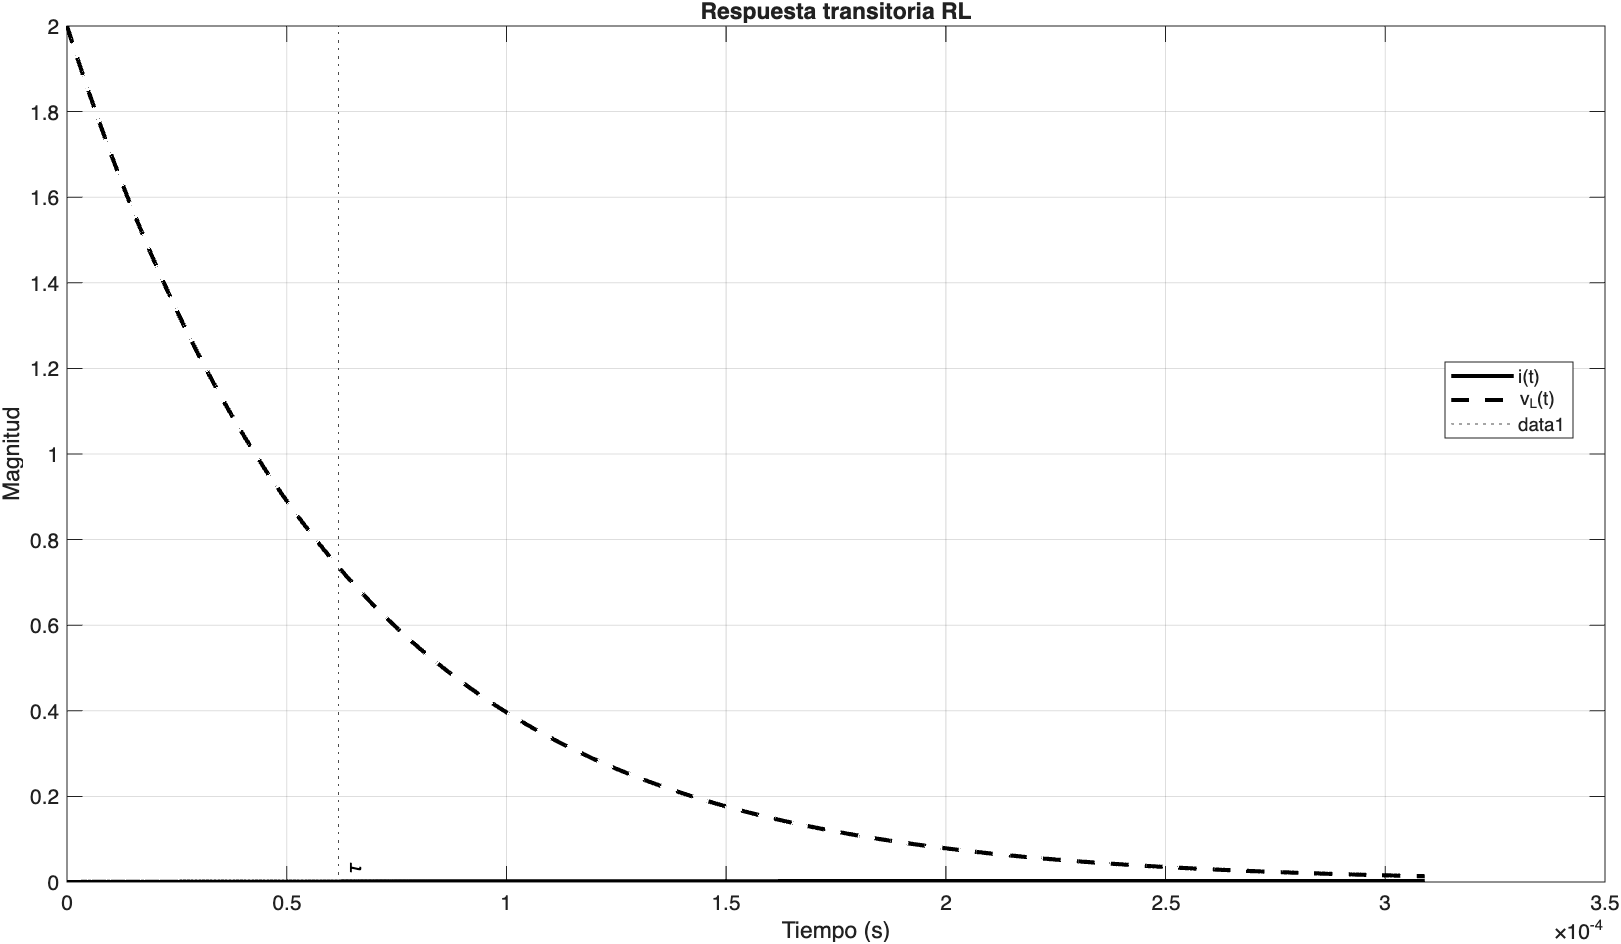
\includegraphics[width=0.75\linewidth]{transitoriaRL.png}
				\caption{Respuesta transitoria RL}
			\end{figure}

\newpage
\section{Conclusiones}
	
	\hspace{0.5cm}El análisis experimental y matemático de los circuitos RC y RL permitió comprobar de manera clara cómo la naturaleza del elemento reactivo (capacitor o inductor) determina el comportamiento dinámico del sistema. 
	
	\hspace{0.5cm}Se confirmó que el capacitor y el inductor no solo almacenan energía de formas distintas, eléctrica y magnética respectivamente, sino que condicionan la respuesta temporal y frecuencial del circuito ante diferentes tipos de excitación.
	
	\hspace{0.5cm}En el dominio del tiempo, ambos circuitos mostraron respuestas exponenciales características de sistemas de prime orden, verificando que la rapidez con la que el sistema alcanza el estado permanente está gobernada por la constante de tiempo $\tau$. 
	Mediante la excitación en DC, se observó que al finalizar el periodo transitorio, el capacitor se comporta físicamente como un circuito abierto, mientras que el inductor actúa como un cortocircuito, validando los modelos teóricos de estado estacionario.
	
	\hspace{0.5cm}El análisis en el dominio de la frecuencia evidenció el desfasamiento entre voltaje y corriente (un adelanto en el caso capacitivo y un atraso en el caso inductivo). 
	Se comprobó experimentalmente que la reactancia capacitiva disminuye conforme aumenta la frecuencia, mientras que la reactancia inductiva aumenta de forma proporcional, lo cual explica su funcionamiento como filtros.
	
	\hspace{0.5cm}Durante la realización de la práctica se redescubrieron conceptos vistos en materias anteriores, lo cual consideramos algo grato, pues ver que todos estos conceptos vistos nos siguen ayudando en la realización de experimentos nos dice que nada de esto será en vano. 
	Se logró cumplir además con los objetivos propuestos sin ningun inconveniente o problema significativo. 
	
\section{Bibliografía}

	\hspace{0.5cm}Soliman, A. (2022). \textit{Natural and Step Response for RL, RC and RLC Circuit} (Lecture 9). BSC 113, Electronics 1, Fall 2022.
	
	\vspace{5pt}
	\hspace{0.5cm}Edminister, J. A., Nahvi, M., \& Lázaro Sánchez, E. (2005). \textit{Circuitos eléctricos y electrónicos} (4a ed.). McGraw-Hill Interamericana.
	
\end{document}